\documentclass[10pt]{beamer}

\usetheme[progressbar=frametitle]{metropolis}
\usepackage{appendixnumberbeamer}

\usepackage{booktabs}

% For removing Figure 1 in figures
\usepackage{caption}

%For linking email and website
\usepackage{hyperref}

%For enumeration as words
\usepackage{blindtext}
\usepackage{enumitem}
\usepackage{geometry}

\usepackage{tikz}
\usepackage{xspace}


\title{Theory of Computation}
\subtitle{Tutorial 3 - DFAs}
\author{Cesare Spinoso-Di Piano}
\date{}

\begin{document}

\maketitle

\begin{frame}{Plan for today}
    \setbeamertemplate{section in toc}[sections numbered]
    \tableofcontents[hideallsubsections]
\end{frame}

\section{Introduction to DFAs}

\begin{frame}{DFAs}
    % Sketch a very rough picture with control unit and input,
    % and explain what this machine and automata in general are
    % suppose to do.

\end{frame}


\begin{frame}[t]{Formal definition of a DFA}
    \textbf{Definition.} A \textbf{\underline{deterministic} finite automaton (DFA)} $M$ is a 5 element tuple $M = (Q, \Sigma, \delta, q_0, F)$ where
    \begin{itemize}
        \item $Q$ is the set of all states
        \item $\Sigma$ is the alphabet
        \item $\delta$ is the transition function $\delta: Q \times \Sigma \rightarrow Q$
        \item $q_0$ is the (\underline{unique}) initial state
        \item $F$ is the set of final states
    \end{itemize}
    A DFA is a machine that takes as input a string and returns either an accept or a reject.
\end{frame}


\begin{frame}{DFAs as language accepters}
    \textbf{Consider a DFA M}\\
    \textbf{Definition.} The language \textbf{L(M)} includes all strings (over the alphabet $\Sigma$) accepted by \textbf{M}\\
    {$L(M)$} = \{strings that drive \textbf{M} to a final state\}\\\bigskip
    Which is defined formally as follows:\\
    $L(M) = \{w\in \Sigma ^*: \delta ^*(q_0,w)\in F\}$, where $\delta ^*$ is extended transition function $\delta ^*: Q\times \Sigma ^*\rightarrow Q$.
\end{frame}


\begin{frame}{Example}
    The following is a DFA \textbf{M} such that \textbf{L(M)} = $\{w \in \{0,1\}^* : w$ starts with a 1\} for $\Sigma = \{0,1\}$.
    \begin{center}
        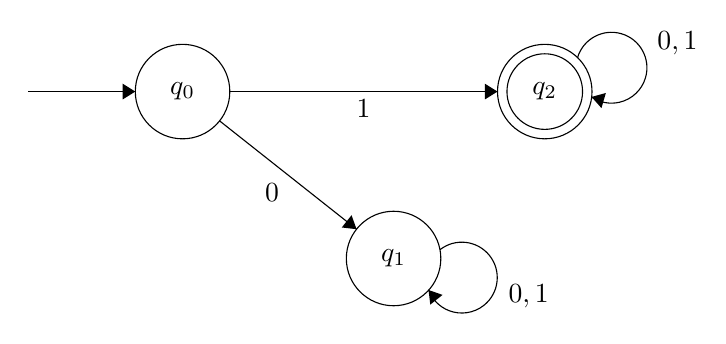
\begin{tikzpicture}[scale=0.2]
            \tikzstyle{every node}+=[inner sep=0pt]
            \draw [black] (18.5,-23.1) circle (3);
            \draw (18.5,-23.1) node {$q_0$};
            \draw [black] (31.9,-33.7) circle (3);
            \draw (31.9,-33.7) node {$q_1$};
            \draw [black] (41.5,-23.1) circle (3);
            \draw (41.5,-23.1) node {$q_2$};
            \draw [black] (41.5,-23.1) circle (2.4);
            \draw [black] (20.85,-24.96) -- (29.55,-31.84);
            \fill [black] (29.55,-31.84) -- (29.23,-30.95) -- (28.61,-31.73);
            \draw (24.19,-28.9) node [below] {$0$};
            \draw [black] (21.5,-23.1) -- (38.5,-23.1);
            \fill [black] (38.5,-23.1) -- (37.7,-22.6) -- (37.7,-23.6);
            \draw (30,-23.6) node [below] {$1$};
            \draw [black] (43.579,-20.953) arc (163.65382:-124.34618:2.25);
            \draw (48.62,-20.06) node [right] {$0,1$};
            \fill [black] (44.47,-23.44) -- (45.1,-24.15) -- (45.38,-23.19);
            \draw [black] (34.837,-33.149) arc (128.35775:-159.64225:2.25);
            \draw (39.17,-36.07) node [right] {$0,1$};
            \fill [black] (34.12,-35.7) -- (34.23,-36.63) -- (35.01,-36.01);
            \draw [black] (8.7,-23.1) -- (15.5,-23.1);
            \fill [black] (15.5,-23.1) -- (14.7,-22.6) -- (14.7,-23.6);
        \end{tikzpicture}
    \end{center}
\end{frame}

\begin{frame}{Example - Tracing input}
    \textbf{L(M)} = $\{w \in \{0,1\}^* : w$ starts with a 1\}\\
    \textbf{Input String: \textcolor{red}{\^{}}101}
    \begin{center}
        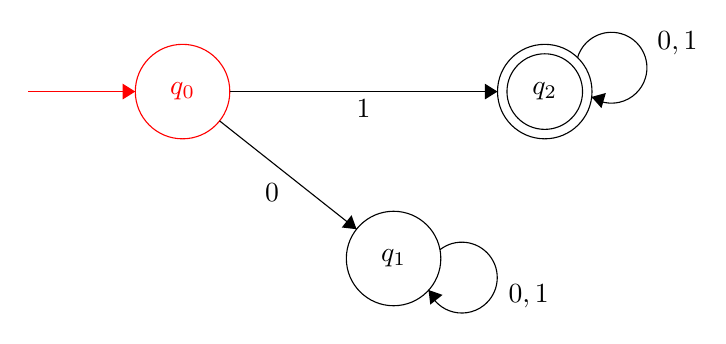
\begin{tikzpicture}[scale=0.2]
            \tikzstyle{every node}+=[inner sep=0pt]
            \draw [red] (18.5,-23.1) circle (3);
            \draw (18.5,-23.1) node [red]{$q_0$};
            \draw [black] (31.9,-33.7) circle (3);
            \draw (31.9,-33.7) node {$q_1$};
            \draw [black] (41.5,-23.1) circle (3);
            \draw (41.5,-23.1) node {$q_2$};
            \draw [black] (41.5,-23.1) circle (2.4);
            \draw [black] (20.85,-24.96) -- (29.55,-31.84);
            \fill [black] (29.55,-31.84) -- (29.23,-30.95) -- (28.61,-31.73);
            \draw (24.19,-28.9) node [below] {$0$};
            \draw [black] (21.5,-23.1) -- (38.5,-23.1);
            \fill [black] (38.5,-23.1) -- (37.7,-22.6) -- (37.7,-23.6);
            \draw (30,-23.6) node [below] {$1$};
            \draw [black] (43.579,-20.953) arc (163.65382:-124.34618:2.25);
            \draw (48.62,-20.06) node [right] {$0,1$};
            \fill [black] (44.47,-23.44) -- (45.1,-24.15) -- (45.38,-23.19);
            \draw [black] (34.837,-33.149) arc (128.35775:-159.64225:2.25);
            \draw (39.17,-36.07) node [right] {$0,1$};
            \fill [black] (34.12,-35.7) -- (34.23,-36.63) -- (35.01,-36.01);
            \draw [red] (8.7,-23.1) -- (15.5,-23.1);
            \fill [red] (15.5,-23.1) -- (14.7,-22.6) -- (14.7,-23.6);
        \end{tikzpicture}
    \end{center}
\end{frame}

\begin{frame}{Example}
    \textbf{L(M)} = $\{w \in \{0,1\}^* : w$ starts with a 1\}\\
    \textbf{Input String: \textcolor{red}101}
    \begin{center}
        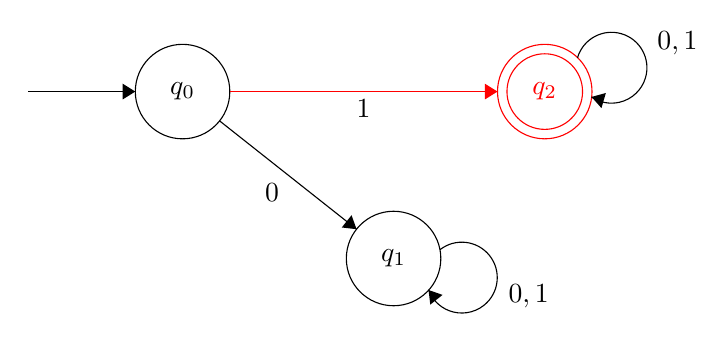
\begin{tikzpicture}[scale=0.2]
            \tikzstyle{every node}+=[inner sep=0pt]
            \draw [black] (18.5,-23.1) circle (3);
            \draw (18.5,-23.1) node {$q_0$};
            \draw [black] (31.9,-33.7) circle (3);
            \draw (31.9,-33.7) node {$q_1$};
            \draw [red] (41.5,-23.1) circle (3);
            \draw (41.5,-23.1) node [red]{$q_2$};
            \draw [red] (41.5,-23.1) circle (2.4);
            \draw [black] (20.85,-24.96) -- (29.55,-31.84);
            \fill [black] (29.55,-31.84) -- (29.23,-30.95) -- (28.61,-31.73);
            \draw (24.19,-28.9) node [below] {$0$};
            \draw [red] (21.5,-23.1) -- (38.5,-23.1);
            \fill [red] (38.5,-23.1) -- (37.7,-22.6) -- (37.7,-23.6);
            \draw (30,-23.6) node [below] {$1$};
            \draw [black] (43.579,-20.953) arc (163.65382:-124.34618:2.25);
            \draw (48.62,-20.06) node [right] {$0,1$};
            \fill [black] (44.47,-23.44) -- (45.1,-24.15) -- (45.38,-23.19);
            \draw [black] (34.837,-33.149) arc (128.35775:-159.64225:2.25);
            \draw (39.17,-36.07) node [right] {$0,1$};
            \fill [black] (34.12,-35.7) -- (34.23,-36.63) -- (35.01,-36.01);
            \draw [black] (8.7,-23.1) -- (15.5,-23.1);
            \fill [black] (15.5,-23.1) -- (14.7,-22.6) -- (14.7,-23.6);
        \end{tikzpicture}
    \end{center}
\end{frame}

\begin{frame}{Example}
    \textbf{L(M)} = $\{w \in \{0,1\}^* : w$ starts with a 1\}\\
    \textbf{Input String: 1\textcolor{red}01}
    \begin{center}
        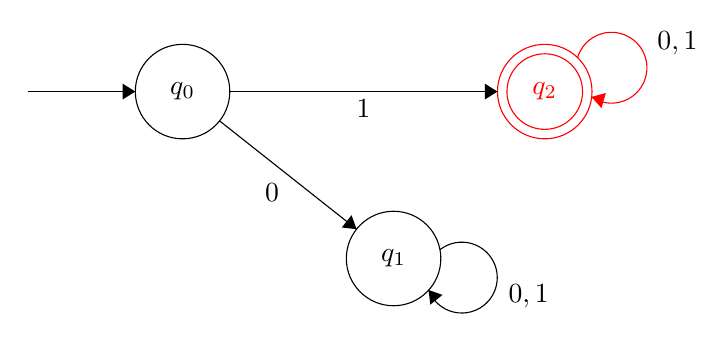
\begin{tikzpicture}[scale=0.2]
            \tikzstyle{every node}+=[inner sep=0pt]
            \draw [black] (18.5,-23.1) circle (3);
            \draw (18.5,-23.1) node {$q_0$};
            \draw [black] (31.9,-33.7) circle (3);
            \draw (31.9,-33.7) node {$q_1$};
            \draw [red] (41.5,-23.1) circle (3);
            \draw (41.5,-23.1) node [red]{$q_2$};
            \draw [red] (41.5,-23.1) circle (2.4);
            \draw [black] (20.85,-24.96) -- (29.55,-31.84);
            \fill [black] (29.55,-31.84) -- (29.23,-30.95) -- (28.61,-31.73);
            \draw (24.19,-28.9) node [below] {$0$};
            \draw [black] (21.5,-23.1) -- (38.5,-23.1);
            \fill [black] (38.5,-23.1) -- (37.7,-22.6) -- (37.7,-23.6);
            \draw (30,-23.6) node [below] {$1$};
            \draw [red] (43.579,-20.953) arc (163.65382:-124.34618:2.25);
            \draw (48.62,-20.06) node [right] {$0,1$};
            \fill [red] (44.47,-23.44) -- (45.1,-24.15) -- (45.38,-23.19);
            \draw [black] (34.837,-33.149) arc (128.35775:-159.64225:2.25);
            \draw (39.17,-36.07) node [right] {$0,1$};
            \fill [black] (34.12,-35.7) -- (34.23,-36.63) -- (35.01,-36.01);
            \draw [black] (8.7,-23.1) -- (15.5,-23.1);
            \fill [black] (15.5,-23.1) -- (14.7,-22.6) -- (14.7,-23.6);
        \end{tikzpicture}
    \end{center}
\end{frame}

\begin{frame}{Example}
    \textbf{L(M)} = $\{w \in \{0,1\}^* : w$ starts with a 1\}\\
    \textbf{Input String: 10\textcolor{red}1}
    \begin{center}
        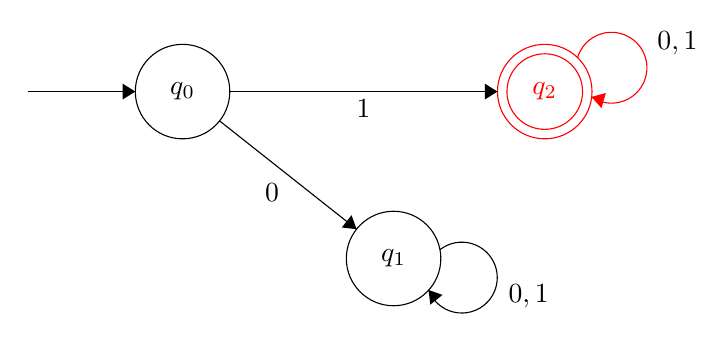
\begin{tikzpicture}[scale=0.2]
            \tikzstyle{every node}+=[inner sep=0pt]
            \draw [black] (18.5,-23.1) circle (3);
            \draw (18.5,-23.1) node {$q_0$};
            \draw [black] (31.9,-33.7) circle (3);
            \draw (31.9,-33.7) node {$q_1$};
            \draw [red] (41.5,-23.1) circle (3);
            \draw (41.5,-23.1) node [red]{$q_2$};
            \draw [red] (41.5,-23.1) circle (2.4);
            \draw [black] (20.85,-24.96) -- (29.55,-31.84);
            \fill [black] (29.55,-31.84) -- (29.23,-30.95) -- (28.61,-31.73);
            \draw (24.19,-28.9) node [below] {$0$};
            \draw [black] (21.5,-23.1) -- (38.5,-23.1);
            \fill [black] (38.5,-23.1) -- (37.7,-22.6) -- (37.7,-23.6);
            \draw (30,-23.6) node [below] {$1$};
            \draw [red] (43.579,-20.953) arc (163.65382:-124.34618:2.25);
            \draw (48.62,-20.06) node [right] {$0,1$};
            \fill [red] (44.47,-23.44) -- (45.1,-24.15) -- (45.38,-23.19);
            \draw [black] (34.837,-33.149) arc (128.35775:-159.64225:2.25);
            \draw (39.17,-36.07) node [right] {$0,1$};
            \fill [black] (34.12,-35.7) -- (34.23,-36.63) -- (35.01,-36.01);
            \draw [black] (8.7,-23.1) -- (15.5,-23.1);
            \fill [black] (15.5,-23.1) -- (14.7,-22.6) -- (14.7,-23.6);
        \end{tikzpicture}
    \end{center}
    The input finishes in a final state, \textbf{M} accepts.
\end{frame}


\begin{frame}{Example}
    \textbf{L(M)} = $\{w \in \{0,1\}^* : w$ starts with a 1\}\\
    \textbf{Input String: \textcolor{red}{\^{}}010}
    \begin{center}
        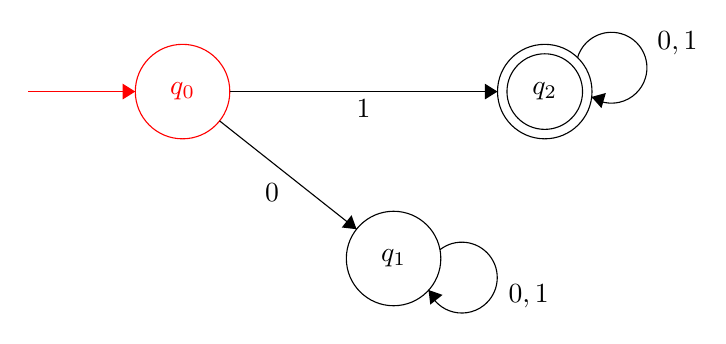
\begin{tikzpicture}[scale=0.2]
            \tikzstyle{every node}+=[inner sep=0pt]
            \draw [red] (18.5,-23.1) circle (3);
            \draw (18.5,-23.1) node [red]{$q_0$};
            \draw [black] (31.9,-33.7) circle (3);
            \draw (31.9,-33.7) node {$q_1$};
            \draw [black] (41.5,-23.1) circle (3);
            \draw (41.5,-23.1) node {$q_2$};
            \draw [black] (41.5,-23.1) circle (2.4);
            \draw [black] (20.85,-24.96) -- (29.55,-31.84);
            \fill [black] (29.55,-31.84) -- (29.23,-30.95) -- (28.61,-31.73);
            \draw (24.19,-28.9) node [below] {$0$};
            \draw [black] (21.5,-23.1) -- (38.5,-23.1);
            \fill [black] (38.5,-23.1) -- (37.7,-22.6) -- (37.7,-23.6);
            \draw (30,-23.6) node [below] {$1$};
            \draw [black] (43.579,-20.953) arc (163.65382:-124.34618:2.25);
            \draw (48.62,-20.06) node [right] {$0,1$};
            \fill [black] (44.47,-23.44) -- (45.1,-24.15) -- (45.38,-23.19);
            \draw [black] (34.837,-33.149) arc (128.35775:-159.64225:2.25);
            \draw (39.17,-36.07) node [right] {$0,1$};
            \fill [black] (34.12,-35.7) -- (34.23,-36.63) -- (35.01,-36.01);
            \draw [red] (8.7,-23.1) -- (15.5,-23.1);
            \fill [red] (15.5,-23.1) -- (14.7,-22.6) -- (14.7,-23.6);
        \end{tikzpicture}
    \end{center}
\end{frame}

\begin{frame}{Example}
    \textbf{L(M)} = $\{w \in \{0,1\}^* : w$ starts with a 1\}\\
    \textbf{Input String: \textcolor{red}010}
    \begin{center}
        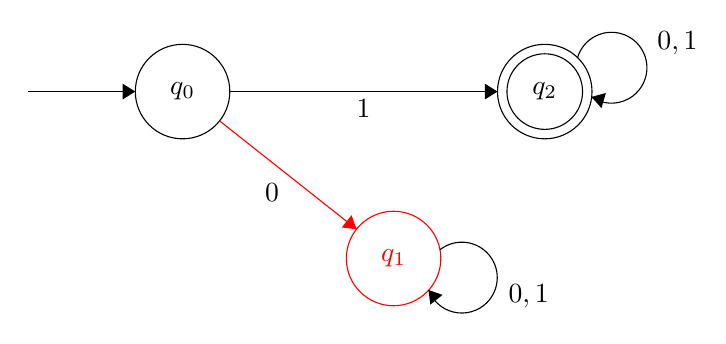
\begin{tikzpicture}[scale=0.2]
            \tikzstyle{every node}+=[inner sep=0pt]
            \draw [black] (18.5,-23.1) circle (3);
            \draw (18.5,-23.1) node {$q_0$};
            \draw [red] (31.9,-33.7) circle (3);
            \draw (31.9,-33.7) node [red]{$q_1$};
            \draw [black] (41.5,-23.1) circle (3);
            \draw (41.5,-23.1) node {$q_2$};
            \draw [black] (41.5,-23.1) circle (2.4);
            \draw [red] (20.85,-24.96) -- (29.55,-31.84);
            \fill [red] (29.55,-31.84) -- (29.23,-30.95) -- (28.61,-31.73);
            \draw (24.19,-28.9) node [below] {$0$};
            \draw [black] (21.5,-23.1) -- (38.5,-23.1);
            \fill [black] (38.5,-23.1) -- (37.7,-22.6) -- (37.7,-23.6);
            \draw (30,-23.6) node [below] {$1$};
            \draw [black] (43.579,-20.953) arc (163.65382:-124.34618:2.25);
            \draw (48.62,-20.06) node [right] {$0,1$};
            \fill [black] (44.47,-23.44) -- (45.1,-24.15) -- (45.38,-23.19);
            \draw [black] (34.837,-33.149) arc (128.35775:-159.64225:2.25);
            \draw (39.17,-36.07) node [right] {$0,1$};
            \fill [black] (34.12,-35.7) -- (34.23,-36.63) -- (35.01,-36.01);
            \draw [black] (8.7,-23.1) -- (15.5,-23.1);
            \fill [black] (15.5,-23.1) -- (14.7,-22.6) -- (14.7,-23.6);
        \end{tikzpicture}
    \end{center}
\end{frame}



\begin{frame}{Example}
    \textbf{L(M)} = $\{w \in \{0,1\}^* : w$ starts with a 1\}\\
    \textbf{Input String: 0\textcolor{red}10}
    \begin{center}
        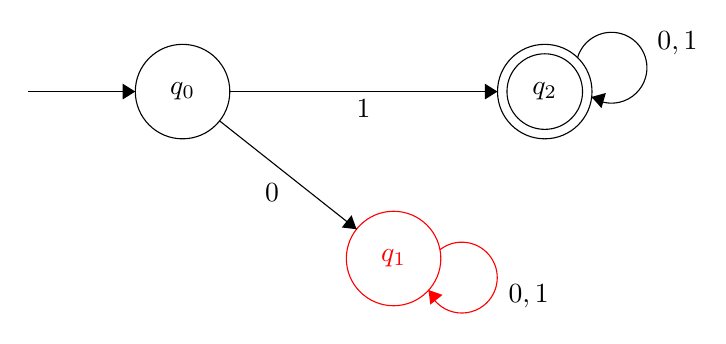
\begin{tikzpicture}[scale=0.2]
            \tikzstyle{every node}+=[inner sep=0pt]
            \draw [black] (18.5,-23.1) circle (3);
            \draw (18.5,-23.1) node {$q_0$};
            \draw [red] (31.9,-33.7) circle (3);
            \draw (31.9,-33.7) node [red]{$q_1$};
            \draw [black] (41.5,-23.1) circle (3);
            \draw (41.5,-23.1) node {$q_2$};
            \draw [black] (41.5,-23.1) circle (2.4);
            \draw [black] (20.85,-24.96) -- (29.55,-31.84);
            \fill [black] (29.55,-31.84) -- (29.23,-30.95) -- (28.61,-31.73);
            \draw (24.19,-28.9) node [below] {$0$};
            \draw [black] (21.5,-23.1) -- (38.5,-23.1);
            \fill [black] (38.5,-23.1) -- (37.7,-22.6) -- (37.7,-23.6);
            \draw (30,-23.6) node [below] {$1$};
            \draw [black] (43.579,-20.953) arc (163.65382:-124.34618:2.25);
            \draw (48.62,-20.06) node [right] {$0,1$};
            \fill [black] (44.47,-23.44) -- (45.1,-24.15) -- (45.38,-23.19);
            \draw [red] (34.837,-33.149) arc (128.35775:-159.64225:2.25);
            \draw (39.17,-36.07) node [right] {$0,1$};
            \fill [red] (34.12,-35.7) -- (34.23,-36.63) -- (35.01,-36.01);
            \draw [black] (8.7,-23.1) -- (15.5,-23.1);
            \fill [black] (15.5,-23.1) -- (14.7,-22.6) -- (14.7,-23.6);
        \end{tikzpicture}
    \end{center}
\end{frame}

\begin{frame}{Example}
    \textbf{L(M)} = $\{w \in \{0,1\}^* : w$ starts with a 1\}\\
    \textbf{Input String: 01\textcolor{red}0}
    \begin{center}
        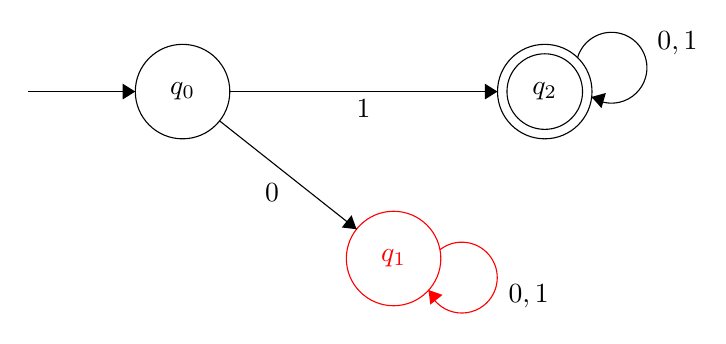
\begin{tikzpicture}[scale=0.2]
            \tikzstyle{every node}+=[inner sep=0pt]
            \draw [black] (18.5,-23.1) circle (3);
            \draw (18.5,-23.1) node {$q_0$};
            \draw [red] (31.9,-33.7) circle (3);
            \draw (31.9,-33.7) node [red]{$q_1$};
            \draw [black] (41.5,-23.1) circle (3);
            \draw (41.5,-23.1) node {$q_2$};
            \draw [black] (41.5,-23.1) circle (2.4);
            \draw [black] (20.85,-24.96) -- (29.55,-31.84);
            \fill [black] (29.55,-31.84) -- (29.23,-30.95) -- (28.61,-31.73);
            \draw (24.19,-28.9) node [below] {$0$};
            \draw [black] (21.5,-23.1) -- (38.5,-23.1);
            \fill [black] (38.5,-23.1) -- (37.7,-22.6) -- (37.7,-23.6);
            \draw (30,-23.6) node [below] {$1$};
            \draw [black] (43.579,-20.953) arc (163.65382:-124.34618:2.25);
            \draw (48.62,-20.06) node [right] {$0,1$};
            \fill [black] (44.47,-23.44) -- (45.1,-24.15) -- (45.38,-23.19);
            \draw [red] (34.837,-33.149) arc (128.35775:-159.64225:2.25);
            \draw (39.17,-36.07) node [right] {$0,1$};
            \fill [red] (34.12,-35.7) -- (34.23,-36.63) -- (35.01,-36.01);
            \draw [black] (8.7,-23.1) -- (15.5,-23.1);
            \fill [black] (15.5,-23.1) -- (14.7,-22.6) -- (14.7,-23.6);
        \end{tikzpicture}
    \end{center}
    The input does not end in a final state, \textbf{M} rejects.
\end{frame}

\begin{frame}[t]{Example}
    \textbf{Example.} Create a DFA that accepts the language $L=\{w\in\{0,1\}^*: w$ contains 00 as a substring\}.
\end{frame}

\section{Regular Languages}
\begin{frame}{Regular Languages}
    \textbf{Definition.} A language $L$ is regular if there exists a DFA $M$ such that $L(M) = L$. One way \textit{to show that a language $L$ is regular is to show there is a DFA $M$ that accepts it}.
\end{frame}

\begin{frame}[t]{Example}
    \textbf{Example.} Show that the language $L = \{a^n : \text{$n$ is a multiple of 2 but not of 3} \}$ ($\Sigma = \{a\}$) is regular.
\end{frame}

\end{document}